\documentclass[./../main_file.tex]{subfiles}

\begin{document}
	
	Trong phần này, nhóm sẽ giới thiệu cách cài đặt và sử dung 3 công cụ của Selenium.
		
	\subsection{Selenium IDE}
	
	Vì Selenium IDE là add-on trên Mozilla Firefox hoặc extension trên Google Chrome, Microsoft Edge nên việc cài đặt Selenium IDE vô cùng đơn giản. Yêu cầu bắt buộc để cài đặt Selenium IDE là máy tính có cài đặt một trong các trình duyệt trên. Nhóm sẽ hướng dẫn các bước cài đặt Selenium IDE trên trình duyệt Google Chrome.
	
	\begin{enumerate}
		\item Tìm kiếm Selenium IDE trên cửa hàng extension của Google Chrome hoặc Firefox (hình \ref{fig:ide_chrome})
		\begin{figure}
			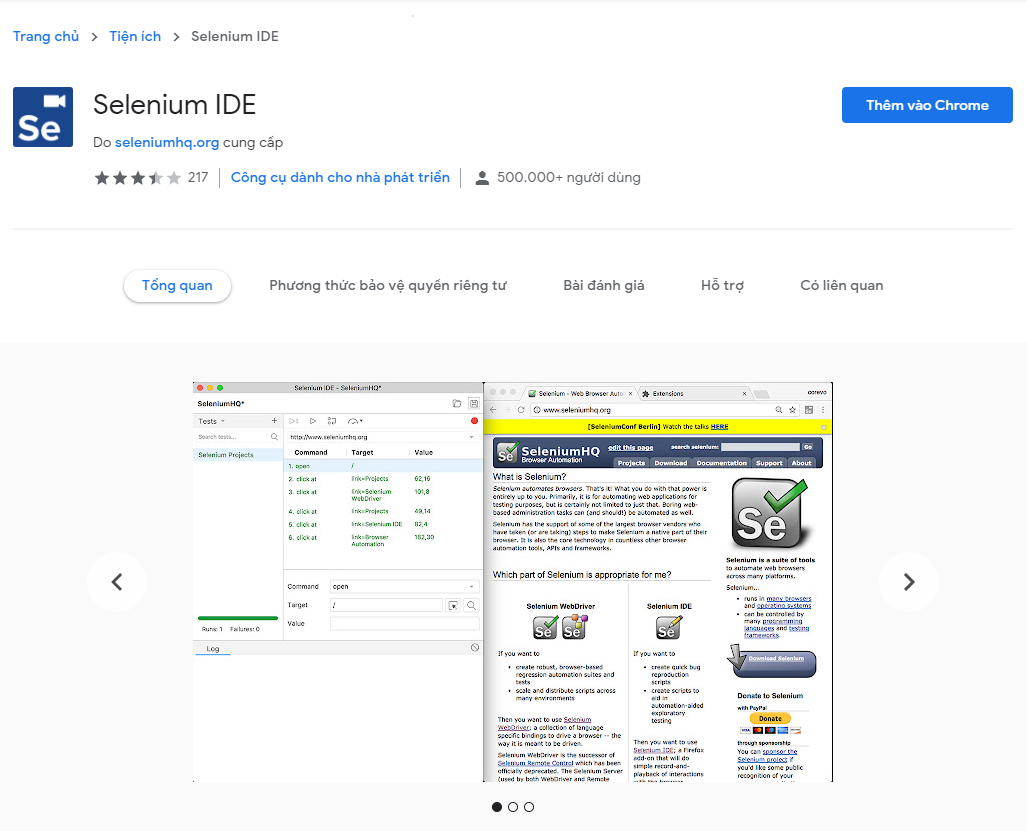
\includegraphics[width=\linewidth]{./images/ide_install.png}
			\caption{Trang của Selenium IDE trên Chrome Web Store}
			\label{fig:ide_chrome}
		\end{figure}
		\item Nhấn “Thêm vào Chrome” để tiến hành cài đặt % (hình \ref{fig:ide_add_to_chrome})
%		\begin{figure}
%			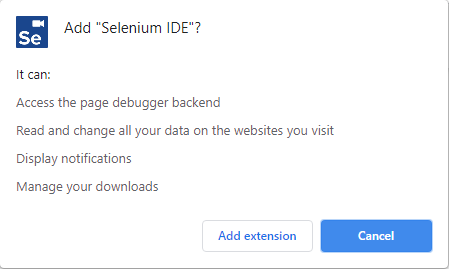
\includegraphics[width=\linewidth]{./images/ide_add_to_chrome.png}
%			\caption{Thêm Selenium IDE vào Chrome}
%			\label{fig:ide_add_to_chrome}
%		\end{figure}
		\item Sau khi cài đặt xong, Selenium IDE sẽ hiển thị trên thanh công cụ. Nhấn vào biểu tượng Selenium IDE để chạy ứng dụng
%		\begin{figure}
%			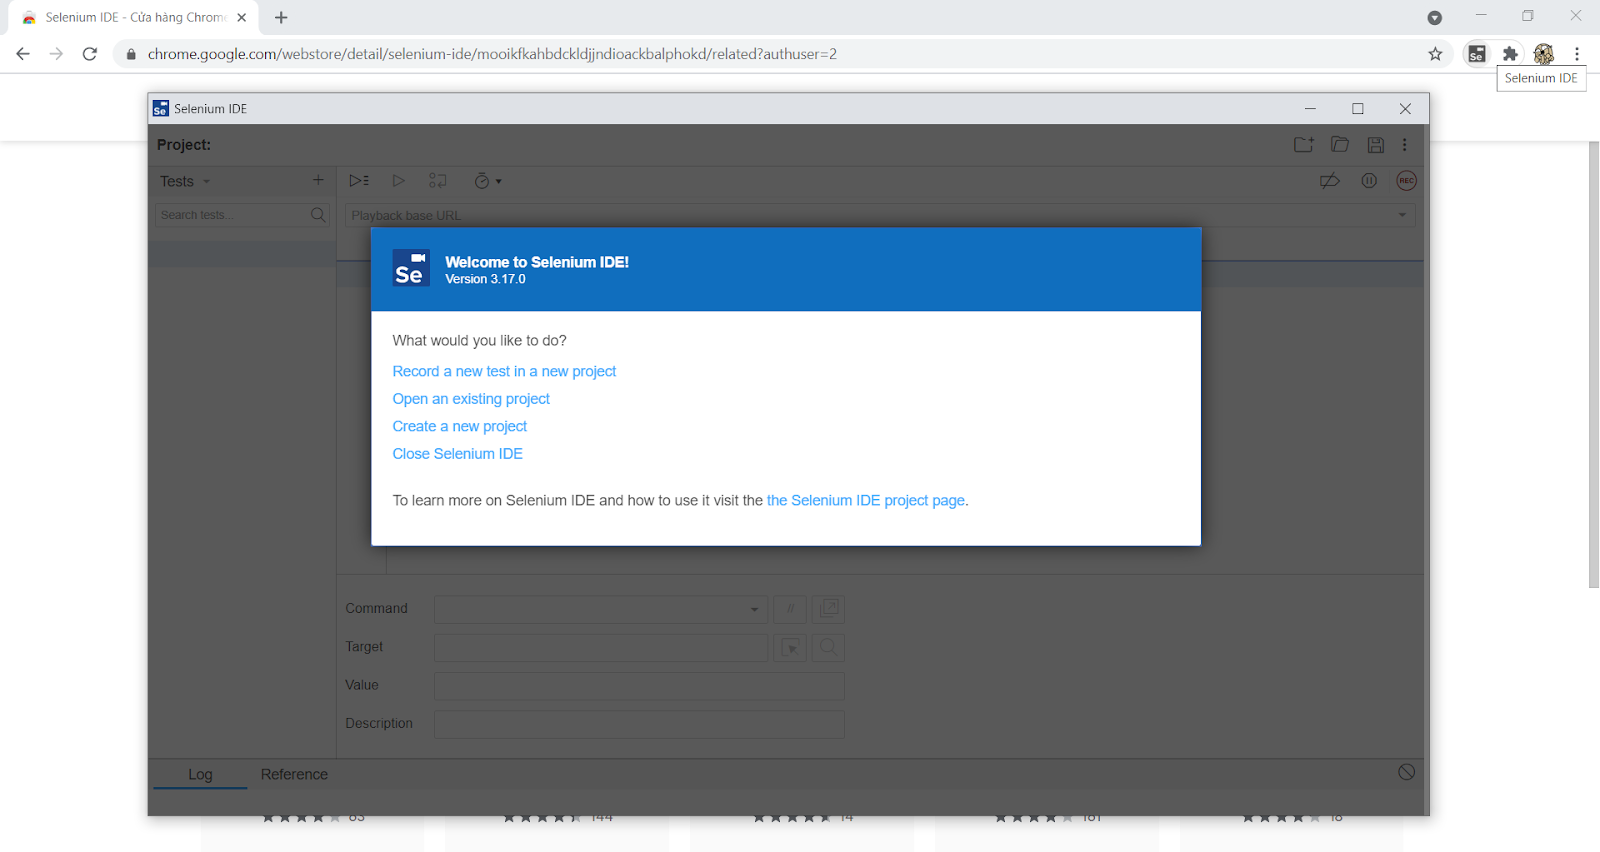
\includegraphics[width=\linewidth]{./images/ide_use.png}
%			\caption{Sử dụng Selenium IDE}
%			\label{fig:ide_use}
%		\end{figure}
	\end{enumerate}
	
\end{document}